\documentclass[entwurf]{uebblatt}
\begin{document}

\maketitle{12}

{\small
Bei den gewöhnlichen reellen Zahlen stehen in ihrer Dezimalschreibweise vor dem
Komma nur endlich viele Ziffern, hinter dem Komma aber gelegentlich unendlich
viele Ziffern. Bei den~$10$-adischen Zahlen ist es genau umgekehrt: Vor dem
Komma dürfen unendlich viele Ziffern stehen, hinter dem Komma dagegen nur
endlich viele. Die Rechenverfahren zur Addition, Subtraktion und
Multiplikation, wie man sie aus der Schule kennt, funktionieren weitestgehend
unverändert. Die Division wird etwas komplizierter. Die~$p$-adischen Zahlen
sind wie die~$10$-adischen, nur dass man die Ziffern~$\{0,\ldots,p-1\}$
verwendet.\par}

\bigskip

\begin{aufgabe}{Spiel und Spaß mit~$10$-adischen Zahlen I}
\begin{enumerate}
\item Was ist~$\ldots 99999 + 1$ in~$\ZZ_{10}$?
\item Schreibe~$2/3$ als~$10$-adische Zahl.
\item Gib ein Element~$x \in \ZZ_{10}$ an, das weder Null noch Eins ist, aber trotzdem
die Identität~$x^2 = x$ erfüllt. Kann ein Grundschulkind die ersten paar
Ziffern von~$x$ bestimmen?
\end{enumerate}
\end{aufgabe}

\begin{aufgabe}{Spiel und Spaß mit~$p$-adischen Zahlen II}
\begin{enumerate}
\item Sei~$n$ eine zu~$p$ teilerfremde ganze Zahl. Zeige, dass~$n$ in~$\ZZ_p$
invertierbar ist.

{\tiny\emph{Tipp.} Hensels Lemma.\par}
\item Berechne $\lim_{n \to \infty} \frac{1}{1 + p^n}$ und $\lim_{n \to \infty}
\frac{p^n}{1 + p^n}$ in~$\RR$ und in~$\ZZ_p$.

{\tiny\emph{Hinweis.} Freestyle-Aufgabe! Mach dir keinen großen Kopf um formale
Rechtfertigung. Es gilt~$\lim_{n \to \infty} p^n = 0$ in~$\ZZ_p$.\par}
\item Seien~$x$ und~$y$ ganze Zahlen. Finde eine Folge~$p$-adischer Zahlen, die
in~$\RR$ gegen~$x$ und in~$\ZZ_p$ gegen~$y$ konvergiert.
\item Gibt es in~$\ZZ_{13}$ eine Quadratwurzel aus~$-1$?
\end{enumerate}
\end{aufgabe}

\begin{aufgabe}{Hensels Lemma}
Sei~$f \in \ZZ[X]$ ein
Polynom, das modulo~$p$ eine einfache Nullstelle besitzt: ein Element~$x_1
\in \ZZ$ mit~$f(x_1) \equiv 0$ modulo~$p$, sodass es ein Element~$y \in \ZZ$
mit~$f'(x_1) y \equiv 1$ modulo~$p$ gibt.
Wir definieren für~$n \geq 1$: $x_{n+1} \defeq x_n - y f(x_n)$.
\begin{enumerate}
\item Zeige für~$n \geq 1$, dass $x_n \equiv x_m \pmod{p^m}$ für~$m < n$ und dass~$f(x_n) \equiv 0 \pmod{p^n}$.

{\tiny\emph{Tipp.} Induktion und Taylorentwicklung.\par}
\item Verwende die Folge~$(x_n)_n$, um eine Nullstelle von~$f$ in~$\ZZ_p$ zu
konstruieren.
\item Unter welchem Namen ist das Konstruktionsverfahren für die~$x_n$ bekannt?
Bewundere die Einheit der Mathematik.
\end{enumerate}
\end{aufgabe}

{\centering\href{https://en.wikipedia.org/wiki/P-adic_number}{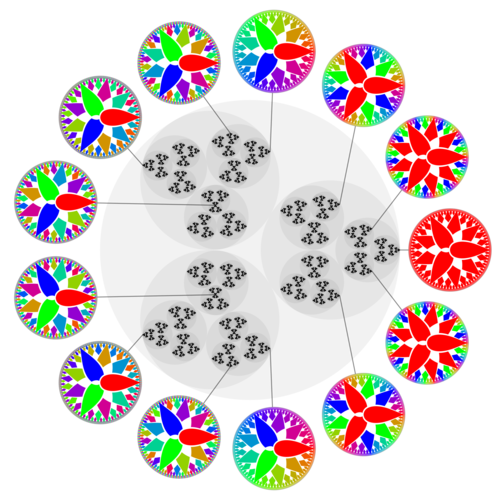
\includegraphics[scale=0.24]{images/p-adic-numbers}}\par}

\end{document}
